%% LaTeX .tex
%% Template para a 2ª Escola Brasileira de Dinâmica de Rotores
%% EBDR 2026
%% 17-18 de setembro de 2026, Uberlândia

\documentclass[10pt,fleqn,a4paper,twoside]{article}
\usepackage{EBDR2026}
\usepackage{array}
% babel removido para evitar option clash com o template
\usepackage[T1]{fontenc}
\usepackage[utf8]{inputenc}
\usepackage{setspace}
\usepackage{indentfirst}
\usepackage{fancyhdr}
\usepackage{titlefoot}
\usepackage{tocloft}
\usepackage{titlesec}
\usepackage{enumitem}
\usepackage[bottom,stable]{footmisc}
\usepackage[hidelinks,pdfstartview=FitH]{hyperref}
\usepackage{graphicx}
\usepackage{caption}
\usepackage{subcaption}
\usepackage{multirow,multicol}
\usepackage[fleqn]{amsmath}
\usepackage{newtxtext,newtxmath}
\usepackage{physics}
\usepackage[brazilian,capitalize]{cleveref}
\usepackage{textcomp}
\usepackage{xcolor}
\usepackage{scalerel}
\usepackage{eqparbox}
\usepackage{longtable}
\usepackage{makecell}
\usepackage{threeparttable}
\usepackage{calc}
\usepackage[locale=FR]{siunitx}
\usepackage{tikz}
\usepackage{pgfplots}
\usepackage{rotating}
\usepackage{empheq}
\usepackage{pdfpages}
\usepackage{float}
\usepackage{etoolbox}
\usepackage{bibentry}
\usepackage{booktabs}
\usepackage{multirow}

\raggedbottom % <--- COMANDO ADICIONADO PARA EVITAR O ESTICAMENTO DA PÁGINA

% Comando alternativo para preencher o cronograma sem depender do \cellcolor (evita conflitos com o template)
\newcommand{\gc}{\textcolor{lightgray}{\rule{6mm}{3mm}}}

% --- CORREÇÃO DO NEGRITO ---
% Redefinindo os comandos do template para evitar o "vazamento" do negrito
\renewcommand{\authors}[1]{{\bfseries #1}}
\renewcommand{\institution}[1]{{\normalfont\small #1}}

% Cabeçalho superior das páginas atualizado com seus dados
\def\shortauthor{Murillo A. B. Sousa, Jessica G. F. Santos, Aldemir A. Cavallini Jr. e Valder Steffen Jr.}
\def\shorttitle{Acoplamento Dinâmico de Rotores Engrenados}

\begin{document}
	\fphead
	
	% Cabeçalho corrigido com \parbox para evitar erros de compilação
	\noindent\hspace*{-2.5mm}\begin{tabular}{||c}
		\parbox{0.97\textwidth}{
			\vspace{2mm}
			{\centering \title{Acoplamento Dinâmico de Rotores Engrenados} \par} \vspace{4mm}
			\authors{Murilo Alvaro Borges de Sousa} \\
			\authors{Jessica Guarato de Freitas Santos} \\
			\authors{Aldemir Aparecido Cavallini Jr.} \\
			\authors{Valder Steffen Jr.} \\
			\institution{Universidade Federal de Uberlândia - UFU} \\
			\institution{murilloabs@ufu.br; jessica.guarato@ufu.br; aacjunior@ufu.br; vsteffen@ufu.br}\\
			\\
			\abstract{\textbf{Resumo.} Este trabalho apresenta uma metodologia matricial baseada em elementos finitos para modelagem e simulação do acoplamento dinâmico de rotores engrenados. Como sistemas de transmissão são essenciais na indústria, compreender sua dinâmica é de fundamental importância. A metodologia foi implementada no \textit{Rotordynamic Open-Source Software} (ROSS), adotando nós com seis graus de liberdade para capturar efeitos translacionais, rotacionais e de torção. A matriz de rigidez de engrenamento considera a geometria de dentes helicoidais. Foi simulado um sistema com dois rotores (motriz e movido) sujeitos a um desbalanceamento, e os resultados temporais comprovaram o acoplamento efetivo entre as direções flexionais e axiais, intrínseco ao perfil helicoidal. Por fim, a abordagem é consistente para análises robustas de caixas de transmissão.}\\
			\\
			\textbf{Palavras-chave:} Dinâmica de Rotores, Engrenagens Helicoidais, MEF, ROSS \vspace{2mm}
		}
	\end{tabular}
	
	\section{INTRODUÇÃO}
	
	Engrenagens transmitem a energia mecânica de motores para diversos equipamentos, como turbomáquinas e geradores, por meio de caixas de transmissão \citep{sousa2026}. Estas são compostas por eixos contendo engrenagens cilíndricas ou cônicas, de dentes retos ou helicoidais. 
	
	Devido aos esforços gerados, a modelagem de sistemas rotativos é essencial para o estudo seguro destes equipamentos \citep{Friswell2010}. Assim, modelar adequadamente o engrenamento e o acoplamento elástico torna-se imprescindível para análises coerentes da dinâmica de rotores acoplados.
	
	\section{FUNDAMENTAÇÃO TEÓRICA}
	
	\subsection{Modelo de rotores flexíveis}
	
	A dinâmica de rotores flexíveis (compostos por eixos, discos, mancais e engrenagens) é modelada calculando-se as energias cinética ($T$) e potencial ($U$) do sistema e aplicando as equações de Lagrange (Eq. \ref{eq_lalanne}) \citep{Lalanne1998}, onde $q_i$ são as coordenadas generalizadas e $Q_{qi}$ as forças não conservativas.
	\begin{equation}
		\frac{\mathrm{d} }{\mathrm{d} t}\left ( \frac{\partial T}{\partial \dot{q_i}} \right )-\frac{\partial T}{\partial q_i} + \frac{\partial U}{\partial q_i}=Q_{qi}
		\label{eq_lalanne}
	\end{equation}
	
	O comportamento dinâmico global resultante é regido pela Eq. \ref{Eq:movement}.
	\begin{equation}
		[M]\{\ddot{q}(t)\}+([C]+\Omega [G])\{\dot{q}(t)\}+[K]\{q(t)\}=\{F(t)\}
		\label{Eq:movement}
	\end{equation}
	
	Onde $[M]$, $[C]$, $[G]$ e $[K]$ representam as matrizes globais de massa, amortecimento, giroscópica e rigidez, respectivamente; $\Omega$ é a velocidade de rotação e $\{F(t)\}$ o vetor de forças externas. O software ROSS \citep{ross, jessica2025} discretiza o modelo adotando seis graus de liberdade por nó (Eq. \ref{Eq:dof}), contemplando translações e rotações nos três eixos. A inserção de engrenagens requer o acréscimo da rigidez de engrenamento aos respectivos nós de acoplamento.
	\vspace*{-0.5cm}
	\begin{equation}
		\{q(t)\} = \{x,y,z, \theta_x, \theta_y, \theta_z\}^{T}
		\label{Eq:dof}
	\end{equation}
	
	\subsection{Acoplamento de rotores engrenados}
	
	A metodologia de acoplamento adotada baseia-se nos trabalhos de \citet{stringer2008, kaplan_paper_2013, kaplan2015}. Para o movimento conjunto, acoplam-se as matrizes nos nós de cada engrenagem ($i$ e $j$), reescrevendo a equação de movimento (Eq.~\ref{Eq:mov-alt}) para contemplar as propriedades de ambos os rotores.
	
	A rigidez de acoplamento $[K_{mesh}]$ atua na direção da linha de ação, não na linha entre centros (Fig.~\ref{fig:mesh_repr}), sendo expressa pela Eq.~\ref{Eq:k_mesh}. As submatrizes ($K_{ii}, K_{jj}, K_{ij}$ e $K_{ji}$) seguem a formulação detalhada na Eq.~\ref{eq:k_matrices} \citep{stringer2008}.
	\begin{figure}%[!ht] % <--- [H] SUBSTITUÍDO POR [!ht]
		\centering
		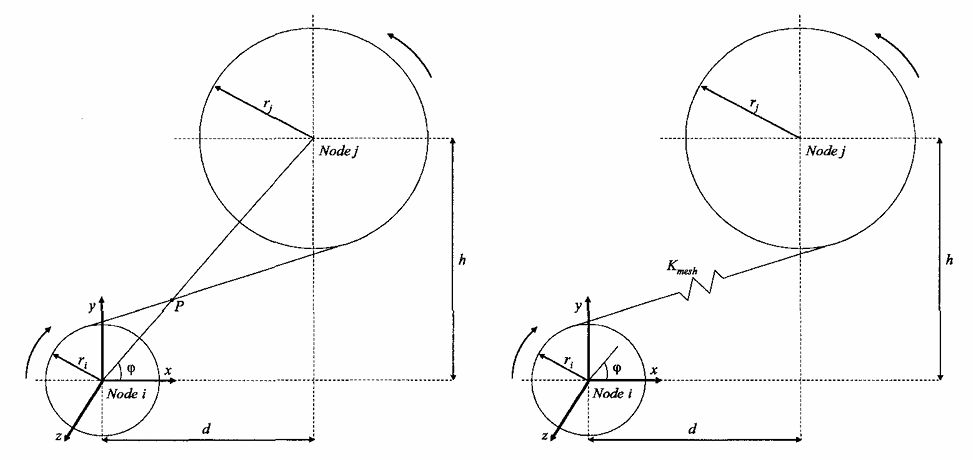
\includegraphics[width=0.6\linewidth]{imagens/gear_mesh_spring.png}
		\caption{Representação do Engrenamento \citep{kaplan2012}}
		\label{fig:mesh_repr}
	\end{figure}
	\begin{equation}
		[M]\{\ddot{q}(t)\}+([C]+\Omega [G])\{\dot{q}(t)\}+([K] + [K_{mesh}])\{q(t)\}=\{F(t)\}
		\label{Eq:mov-alt}
	\end{equation}
%	\vspace*{-0.5cm}
	\begin{equation}
		[K_{mesh}]
		\begin{Bmatrix}
			q_i \\
			q_j
		\end{Bmatrix}
		= K_{g}
		\begin{bmatrix}
			[K_{ii}] & [K_{ij}] \\
			[K_{ji}] & [K_{jj}]
		\end{bmatrix}
		\begin{Bmatrix}
			q_i \\
			q_j
		\end{Bmatrix}
		\label{Eq:k_mesh}
	\end{equation}
%	\vspace*{-0.5cm}
	\begin{equation}
		\label{eq:k_matrices}
		\begin{gathered}
			\resizebox{\linewidth}{!}{
				$K_{ii} = 
				\begin{bmatrix}
					(s\varphi c\phi_x + c\varphi c\phi_y)^2 & & & & & \text{sym} \\
					(s\varphi c\phi_x + c\varphi c\phi_y)(s\varphi c\phi_y - c\varphi c\phi_x) & (s\varphi c\phi_y - c\varphi c\phi_x)^2 & & & & \\
					c\phi_z(s\varphi c\phi_x + c\varphi c\phi_y) & c\phi_z(s\varphi c\phi_y - c\varphi c\phi_x) & c\phi_z^2 & & & \\
					s\varphi c\phi_z r_i(s\varphi c\phi_x + c\varphi c\phi_y) & s\varphi c\phi_z r_i(s\varphi c\phi_y - c\varphi c\phi_x) & s\varphi c\phi_z^2 r_i & (s\varphi c\phi_z r_i)^2 & & \\
					-c\varphi c\phi_z r_i(s\varphi c\phi_x + c\varphi c\phi_y) & -c\varphi c\phi_z r_i(s\varphi c\phi_y - c\varphi c\phi_x) & -c\varphi c\phi_z^2 r_i & -c\varphi s\varphi(c\phi_z r_i)^2 & (c\varphi c\phi_z r_i)^2 & \\
					-c\phi_x r_i(s\varphi c\phi_x + c\varphi c\phi_y) & -c\phi_x r_i(s\varphi c\phi_y - c\varphi c\phi_x) & -c\phi_x c\phi_z r_i & -s\varphi c\phi_x c\phi_z r_i^2 & c\varphi c\phi_x c\phi_z r_i^2 & (c\phi_x r_i)^2
				\end{bmatrix}$
			}
			\\[1.5em]
			\resizebox{\linewidth}{!}{
				$K_{ji} = 
				\begin{bmatrix}
					-(s\varphi c\phi_x + c\varphi c\phi_y)^2 & [K_{ji}]_{2,1} & [K_{ji}]_{3,1} & -s\varphi c\phi_z r_i(s\varphi c\phi_x + c\varphi c\phi_y) & c\varphi c\phi_z r_i(s\varphi c\phi_x + c\varphi c\phi_y) & c\phi_x r_i(s\varphi c\phi_x + c\varphi c\phi_y) \\
					-(s\varphi c\phi_x + c\varphi c\phi_y)(s\varphi c\phi_y - c\varphi c\phi_x) & -(s\varphi c\phi_y - c\varphi c\phi_x)^2 & [K_{ji}]_{3,2} & -s\varphi c\phi_z r_i(s\varphi c\phi_y - c\varphi c\phi_x) & c\varphi c\phi_z r_i(s\varphi c\phi_y - c\varphi c\phi_x) & c\phi_x r_i(s\varphi c\phi_y - c\varphi c\phi_x) \\
					-c\phi_z(s\varphi c\phi_x + c\varphi c\phi_y) & -c\phi_z(s\varphi c\phi_y - c\varphi c\phi_x) & -c\phi_z^2 & -s\varphi c\phi_z^2 r_i & c\varphi c\phi_z^2 r_i & c\phi_x c\phi_z r_i \\
					-s\varphi c\phi_z r_j(s\varphi c\phi_x + c\varphi c\phi_y) & -s\varphi c\phi_z r_j(s\varphi c\phi_y - c\varphi c\phi_x) & -s\varphi c\phi_z^2 r_j & -(s\varphi c\phi_z)^2 r_i r_j & c\varphi s\varphi c\phi_z^2 r_i r_j & s\varphi c\phi_x c\phi_z r_i r_j \\
					c\varphi c\phi_z r_j(s\varphi c\phi_x + c\varphi c\phi_y) & c\varphi c\phi_z r_j(s\varphi c\phi_y - c\varphi c\phi_x) & c\varphi c\phi_z^2 r_j & c\varphi s\varphi c\phi_z^2 r_i r_j & -(c\varphi c\phi_z)^2 r_i r_j & -c\varphi c\phi_x c\phi_z r_i r_j \\
					-c\phi_x r_j(s\varphi c\phi_x + c\varphi c\phi_y) & -c\phi_x r_j(s\varphi c\phi_y - c\varphi c\phi_x) & -c\phi_x c\phi_z r_j & -s\varphi c\phi_x c\phi_z r_i r_j & c\varphi c\phi_x c\phi_z r_i r_j & c\phi_x^2 r_i r_j
				\end{bmatrix}$
			}
			\\[1.5em]
			\resizebox{\linewidth}{!}{
				$K_{jj} = 
				\begin{bmatrix}
					(s\varphi c\phi_x + c\varphi c\phi_y)^2 & & & & & \text{sym} \\
					(s\varphi c\phi_x + c\varphi c\phi_y)(s\varphi c\phi_y - c\varphi c\phi_x) & (s\varphi c\phi_y - c\varphi c\phi_x)^2 & & & & \\
					c\phi_z(s\varphi c\phi_x + c\varphi c\phi_y) & c\phi_z(s\varphi c\phi_y - c\varphi c\phi_x) & c\phi_z^2 & & & \\
					s\varphi c\phi_z r_j(s\varphi c\phi_x + c\varphi c\phi_y) & s\varphi c\phi_z r_j(s\varphi c\phi_y - c\varphi c\phi_x) & s\varphi c\phi_z^2 r_j & (s\varphi c\phi_z r_j)^2 & & \\
					-c\varphi c\phi_z r_j(s\varphi c\phi_x + c\varphi c\phi_y) & -c\varphi c\phi_z r_j(s\varphi c\phi_y - c\varphi c\phi_x) & -c\varphi c\phi_z^2 r_j & -c\varphi s\varphi(c\phi_z r_j)^2 & (c\varphi c\phi_z r_j)^2 & \\
					c\phi_x r_j(s\varphi c\phi_x + c\varphi c\phi_y) & c\phi_x r_j(s\varphi c\phi_y - c\varphi c\phi_x) & c\phi_x c\phi_z r_j & s\varphi c\phi_x c\phi_z r_j^2 & -c\phi_x c\phi_z r_j^2 & (c\phi_x r_j)^2
				\end{bmatrix}$
			}
		\end{gathered}
	\end{equation}
	\begin{gather*}
		\begin{alignedat}{2}
			s\varphi &= \sin\varphi, &\qquad s\varphi^2 &= (\sin\varphi)^2 \\
			c\varphi &= \cos\varphi, &\qquad c\varphi^2 &= (\cos\varphi)^2
		\end{alignedat} %\\[1ex] 
		\hspace{1cm}
		\begin{alignedat}{3}
			\cos\phi_x &= \cos\beta \cos\alpha_n &\qquad \cos\phi_y &= \sin\alpha_n &\qquad \cos\phi_z &= \sin\beta \sin\alpha_n
		\end{alignedat}
	\end{gather*}
	
	Onde $\varphi$ é o ângulo de orientação entre engrenagens, $\beta$ o ângulo de hélice e $\alpha_n$ o ângulo de pressão normal. Os ângulos $\phi_x, \phi_y$ e $\phi_z$ decompõem a força de contato conforme a Fig.~\ref{fig:force_component}.
	\begin{figure}[!ht] % <--- [H] SUBSTITUÍDO POR [!ht]
		\centering
		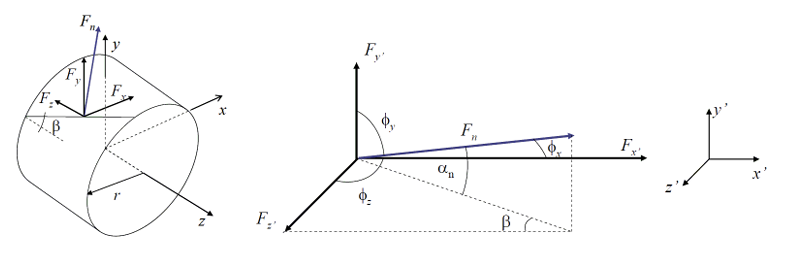
\includegraphics[width=0.7\linewidth]{imagens/force_component.png}
		\caption{Decomposição das forças no ponto de contato \citep{kaplan_paper_2013}.}
		\label{fig:force_component}
	\end{figure}
	
	A rigidez do engrenamento na linha de ação ($K_g$) é calculada assumindo que a flexibilidade dos dentes predomina sobre a do corpo da engrenagem (Eq.~\ref{Eq:Kg}), onde $c$ é a razão de contato, $w$ a largura dos dentes e $E_1, E_2$ os módulos de elasticidade \citep{kaplan2015}.
	\begin{equation}
		K_g = \frac{c w E_1 E_2}{9(E_1+E_2)}
		\label{Eq:Kg}
	\end{equation}
	
	\section{METODOLOGIA}
	Foi desenvolvido um modelo computacional com nós de seis graus de liberdade para simular rotores acoplados. O sistema consiste em dois rotores de aço (Rotor 1 motriz, Rotor 2 movido), engrenados através de engrenagens helicoidais com $25^\circ$ de inclinação, detalhados na Tabela \ref{tab:parametros_multirotor}.
	
	\begin{table}[H] % <--- [H] SUBSTITUÍDO POR [!ht]
		\centering
		\caption{Resumo dos Parâmetros Físicos e de Simulação}
		\label{tab:parametros_multirotor}
		\renewcommand{\arraystretch}{1.2} 
		\begin{tabular}{@{}llcc@{}}
			\toprule
			\textbf{Subsistema} & \textbf{Parâmetro} & \textbf{Rotor 1 (Motriz)} & \textbf{Rotor 2 (Movido)} \\ \midrule
			
			\multirow{4}{*}{\textbf{Eixos}} 
			& Material & \multicolumn{2}{c}{Aço (Padrão ROSS)} \\
			& Comprimento Total & 0,5 m & 0,5 m \\
			& Diâmetro Externo & 0,05 m & 0,05 m \\
			& Diâmetro Interno & 0,0 m (Maciço) & 0,0 m (Maciço) \\ \midrule
			
			\multirow{6}{*}{\textbf{Engrenagens}} 
			& Nó de Posicionamento & Nó 1 & Nó 1 \\
			& Número de Dentes ($Z$) & 30 & 60 \\
			& Diâmetro Primitivo ($d_p$) & 0,15 m & 0,30 m \\
			& Largura do Dente ($b$) & 0,04 m & 0,04 m \\
			& Ângulo de Pressão ($\alpha$) & \multicolumn{2}{c}{$20^\circ$} \\
			& Ângulo de Hélice ($\beta$) & \multicolumn{2}{c}{$25^\circ$} \\ \midrule
			
			\multirow{2}{*}{\textbf{Mancais}} 
			& Rigidez ($K_{xx}, K_{yy}, K_{zz}$) & \multicolumn{2}{c}{$10^7, 1.5 \times 10^7, 10^7$ N/m} \\
			& Amortecimento ($C_{xx}, C_{yy}, C_{zz}$) & \multicolumn{2}{c}{$500, 800, 500$ N.s/m} \\ \midrule
			
			\multirow{2}{*}{\textbf{MultiRotor}} 
			& Nós Acoplados & \multicolumn{2}{c}{Nó 1 (Rotor 1) $\leftrightarrow$ Nó 1 (Rotor 2)} \\
			& Ângulo de Orientação & \multicolumn{2}{c}{$0,0$ rad (Alinhamento Horizontal)} \\ \midrule
			
			\multirow{2}{*}{\textbf{Desbalanceamento}} 
			& Magnitude & 0,005 kg.m & - \\
			& Local de Aplicação & Engrenagem 1 & - \\ \midrule
			
			\multirow{3}{*}{\textbf{Simulação}} 
			& Rotação de Operação & \multicolumn{2}{c}{300 rad/s ($\sim$ 2865 RPM no Rotor 1)} \\
			& Tempo Total / Discret. & \multicolumn{2}{c}{0,5 s / 1000 passos} \\ 
			\bottomrule
		\end{tabular}
	\end{table}
	
	Para avaliar a resposta, aplicou-se um desbalanceamento de $0,005$ kg.m na Engrenagem 1, atuando como excitação harmônica. A simulação integrou 0,5 segundos, mantendo rotação constante no rotor motriz.
	
	\section{RESULTADOS E DISCUSSÃO}
	
	A Figura \ref{fig:response} apresenta a resposta vibratória em regime permanente (de 0,35 a 0,50 segundos). A análise das respostas translacionais ($X$ e $Y$) evidencia o acoplamento entre os rotores. A excitação gerada pelo desbalanceamento no motriz é transmitida à Engrenagem 2 pela linha de ação.
	
	O resultado mais relevante habilitado por esta formulação ocorre no deslocamento $Z$. Devido ao ângulo de hélice ($\beta = 25^\circ$), surge um componente de força axial durante o contato, gerando vibrações acopladas que não ocorreriam em dentes retos.
	
	As respostas rotacionais e torcionais ($R_x$, $R_y$ e $R_z$) evidenciam o forte acoplamento dinâmico entre os eixos. Um comportamento de destaque ocorre em $R_x$, onde as duas engrenagens oscilam em fase. 
	Esse sincronismo decorre pelo fato da engrenagem 2 estar posicionada ao longo do eixo $x$, com relação à engrenagem 1. Caso o posicionamento do Rotor 2 fosse na posição $y$ a variável $R_y$ que estaria em fase.
%	Isso acontece devido ao efeito giroscópico: embora a engrenagem movida gire no sentido contrário e seja "dobrada" em direções opostas em $R_y$ devido ao empuxo axial, essas duas inversões físicas se anulam. Como resultado, o momento giroscópico atua na mesma direção espacial para ambas as engrenagens.
%	Esse fenômeno é um resultado direto do acoplamento giroscópico dos rotores. Na mecânica do engrenamento helicoidal, a componente de empuxo axial gera momentos fletores de sentidos opostos em cada eixo, induzindo deflexões angulares contrárias na direção $R_y$. Simultaneamente, a cinemática do engrenamento externo impõe à engrenagem movida uma velocidade angular reversa. Pela formulação da dinâmica de rotores, o momento giroscópico reativo é proporcional ao produto da velocidade de rotação pela taxa de deflexão fletora transversal. Como o rotor movido sofre uma dupla inversão vetorial --- rotação oposta e flexão fletora oposta ---, os sinais algébricos se cancelam. Consequentemente, os momentos giroscópicos induzidos tornam-se colineares e atuam no mesmo sentido espacial, forçando o sistema a oscilar em fase na direção $R_x$.
	 Além disso, nota-se que o rotor movido vibra de forma mais lenta, o que é totalmente coerente com sua velocidade de rotação reduzida pela metade, validando a relação de transmissão do sistema ($Z_1/Z_2 = 0,5$).
	
	\begin{figure}[H] % <--- [H] SUBSTITUÍDO POR [!ht]
		\centering
		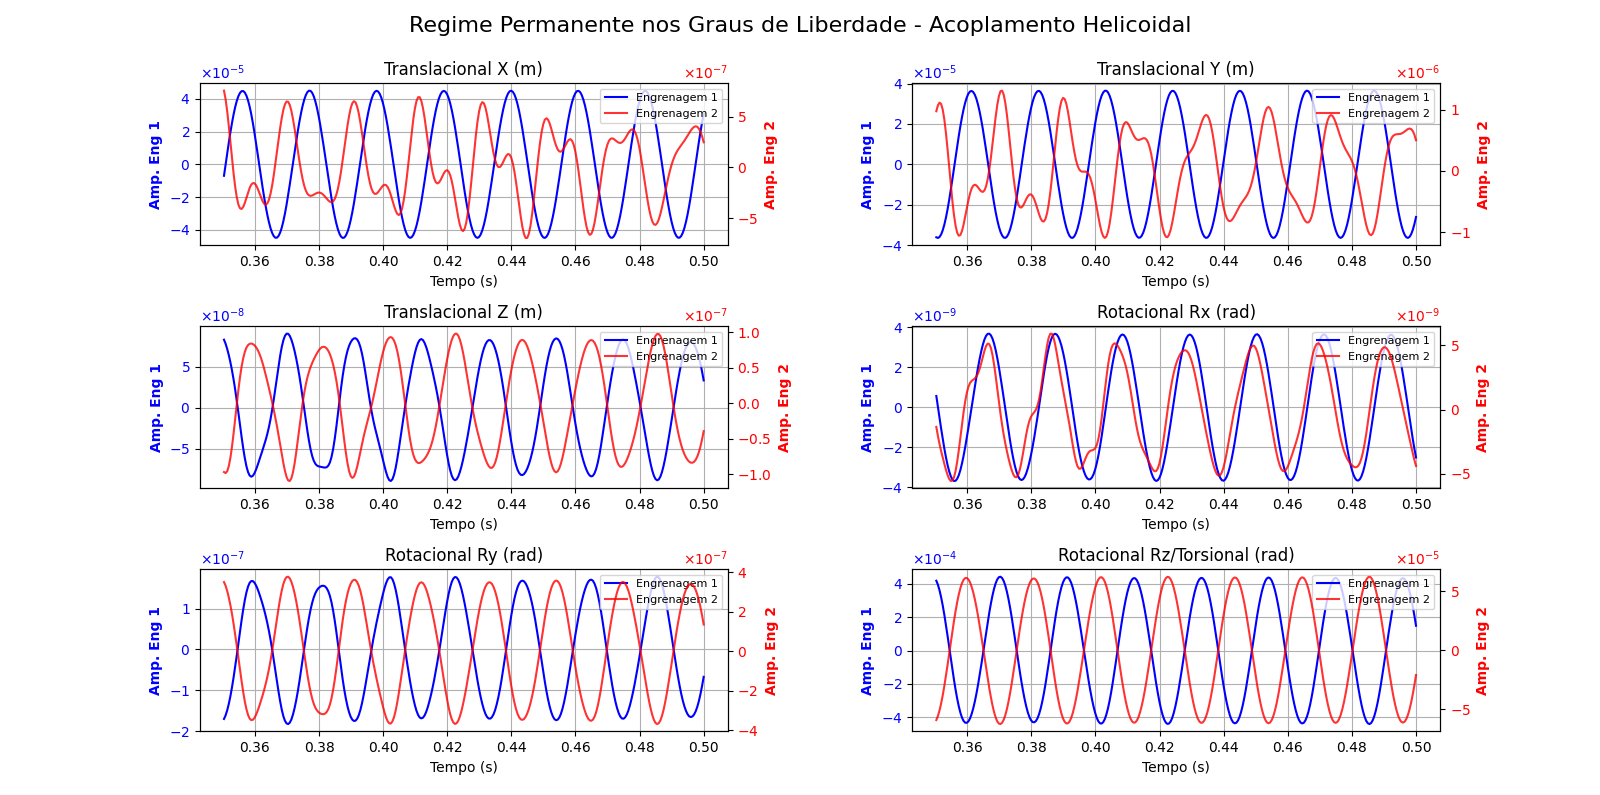
\includegraphics[width=\linewidth]{imagens/response.png}
		\caption{Resposta vibratória nos seis graus de liberdade para as engrenagens acopladas.}
		\label{fig:response}
	\end{figure}
	
%	Os comportamentos rotacionais e torcionais ($Rx$, $Ry$ e $Rz$) reforçam o acoplamento dinâmico. Adicionalmente, o rotor movido oscila com frequências características e fases influenciadas por sua velocidade angular inferior, confirmando a cinemática regida pela relação de transmissão ($Z_1/Z_2 = 0,5$).
	
	\section{CONCLUSÃO}	
	A formulação matricial com nós de seis graus de liberdade demonstrou ser capaz de realizar o acoplamento dinâmico por engrenagens helicoidais. Os resultados comprovaram a propagação da excitação primária, com destaque para a captura das vibrações axiais inerentes a perfis helicoidais. A transferência integrada de forças (radiais, axiais e momentos torsores) utilizada no modelo presente \textit{software} ROSS é uma ferramenta confiável para análise de projetos em caixas de transmissão.
	
	\section{AGRADECIMENTOS}
	Os autores agradecem o suporte financeiro de órgãos de fomento à pesquisa e a infraestrutura oferecida pela UFU.
	
	\section{REFERÊNCIAS}
	\bibliographystyle{EBDR2026}
	\renewcommand{\refname}{}
	\bibliography{bibfile}
	
	\section{TERMO DE RESPONSABILIDADE}
	O(s) autor(es) é (são) o(s) único(s) responsável(is) pelo conteúdo publicado neste artigo.
	
\end{document}